%%%%%%%%%%%%%%%%%%%%%%%%%%%%%%%%%%%%%%%%%%%%%%%%%%%%%%%%%%%%%%%%%%%%%%%%%%%%%%%%%
% Author: First Name Last Name
% Type: Semester/Master Thesis
% Title: Thesis Title
%%%%%%%%%%%%%%%%%%%%%%%%%%%%%%%%%%%%%%%%%%%%%%%%%%%%%%%%%%%%%%%%%%%%%%%%%%%%%%%%%

\documentclass[pdflatex,11pt,a4paper,twoside,titlepage]{scrbook}

%---------packages------------------------------------------------------

\usepackage[english]{babel}
\usepackage[latin1]{inputenc}
\usepackage{a4wide}

\usepackage{amsmath}
\usepackage{amsfonts}
\usepackage{amssymb}
\usepackage{mathcomp}

%\addtokomafont{disposition}{\rmfamily}				% uncomment for serif fonts for headings KOMA classes
\usepackage[hang,labelfont=bf]{caption}				% configure captions of images, tables etc.
%\usepackage[footnotesize,sl,SL,hang,tight]{subfigure}		% helpful package for aligning figures next to each other
%\usepackage{captcont}						% continue sufigures over several pages

\usepackage{verbatim}
\usepackage{booktabs}							% publication quality tables for LaTeX
%\usepackage{multirow}						% cells in tables can span multiple rows
%\usepackage{rotating}
\usepackage{fancyhdr}

\usepackage[pdftex]{color,graphicx}
%\usepackage[hang]{caption}
\usepackage{subfigure}
\usepackage{color}
\usepackage{float}
\usepackage{hyperref}
\usepackage{listings}
\lstset{keywordstyle=\color{blue}\bfseries\emph, breaklines=true, breakatwhitespace=false}
\lstset{language=C, basicstyle=\footnotesize, commentstyle=\color{green}}
\hypersetup
{
pdftitle = {Thesis Title},
pdfauthor = {Name},
colorlinks = {true},
hypertexnames={true},
plainpages={false},
linkcolor={black},
citecolor={black},
filecolor={black},
urlcolor={black},
anchorcolor={black},
menucolor={black},
breaklinks={true}
}

%\setlength{\textwidth}{15cm}
%\setlength{\textheight}{22.0cm}
%\setlength{\oddsidemargin}{0.75cm}
%\setlength{\evensidemargin}{-0.3cm}
%\setlength{\topmargin}{-0.2cm}			% Distance between page top and header
\setlength{\headheight}{15pt}
%\setlength{\parskip}{1.5explus0.5ex}
%\setlength{\parindent}{0pt}				% \noindent
%\renewcommand{\baselinestretch}{1.2}		% Line distance
%\setcounter{secnumdepth}{3}			% Displays Section number down to 3 ranks
%\setcounter{tocdepth}{3}

\newcommand{\clearemptydoublepage}{\newpage{\pagestyle{empty}\cleardoublepage}}
\newcommand{\st}{\stackrel{*}}

%---------document------------------------------------------------------

\begin{document}

\frontmatter

\thispagestyle{empty}
\enlargethispage{2cm} 

\begin{center}
		\vspace*{-3.3cm}
    \rule{\linewidth}{0.5pt} \\
\end{center}


\includegraphics[width=.4\textwidth]{ethlogo}
\vspace{-1.2cm} 

\begin{center}
		\vspace*{0.4cm}
    \rule{\linewidth}{0.5pt} \\
\end{center}


\begin{center}
  \vspace*{.8cm}
  \LARGE \bfseries \boldmath
 Thesis Title
  \vspace*{0.5cm} \unboldmath
\end{center}


\begin{figure}[htb!]
	\centering
  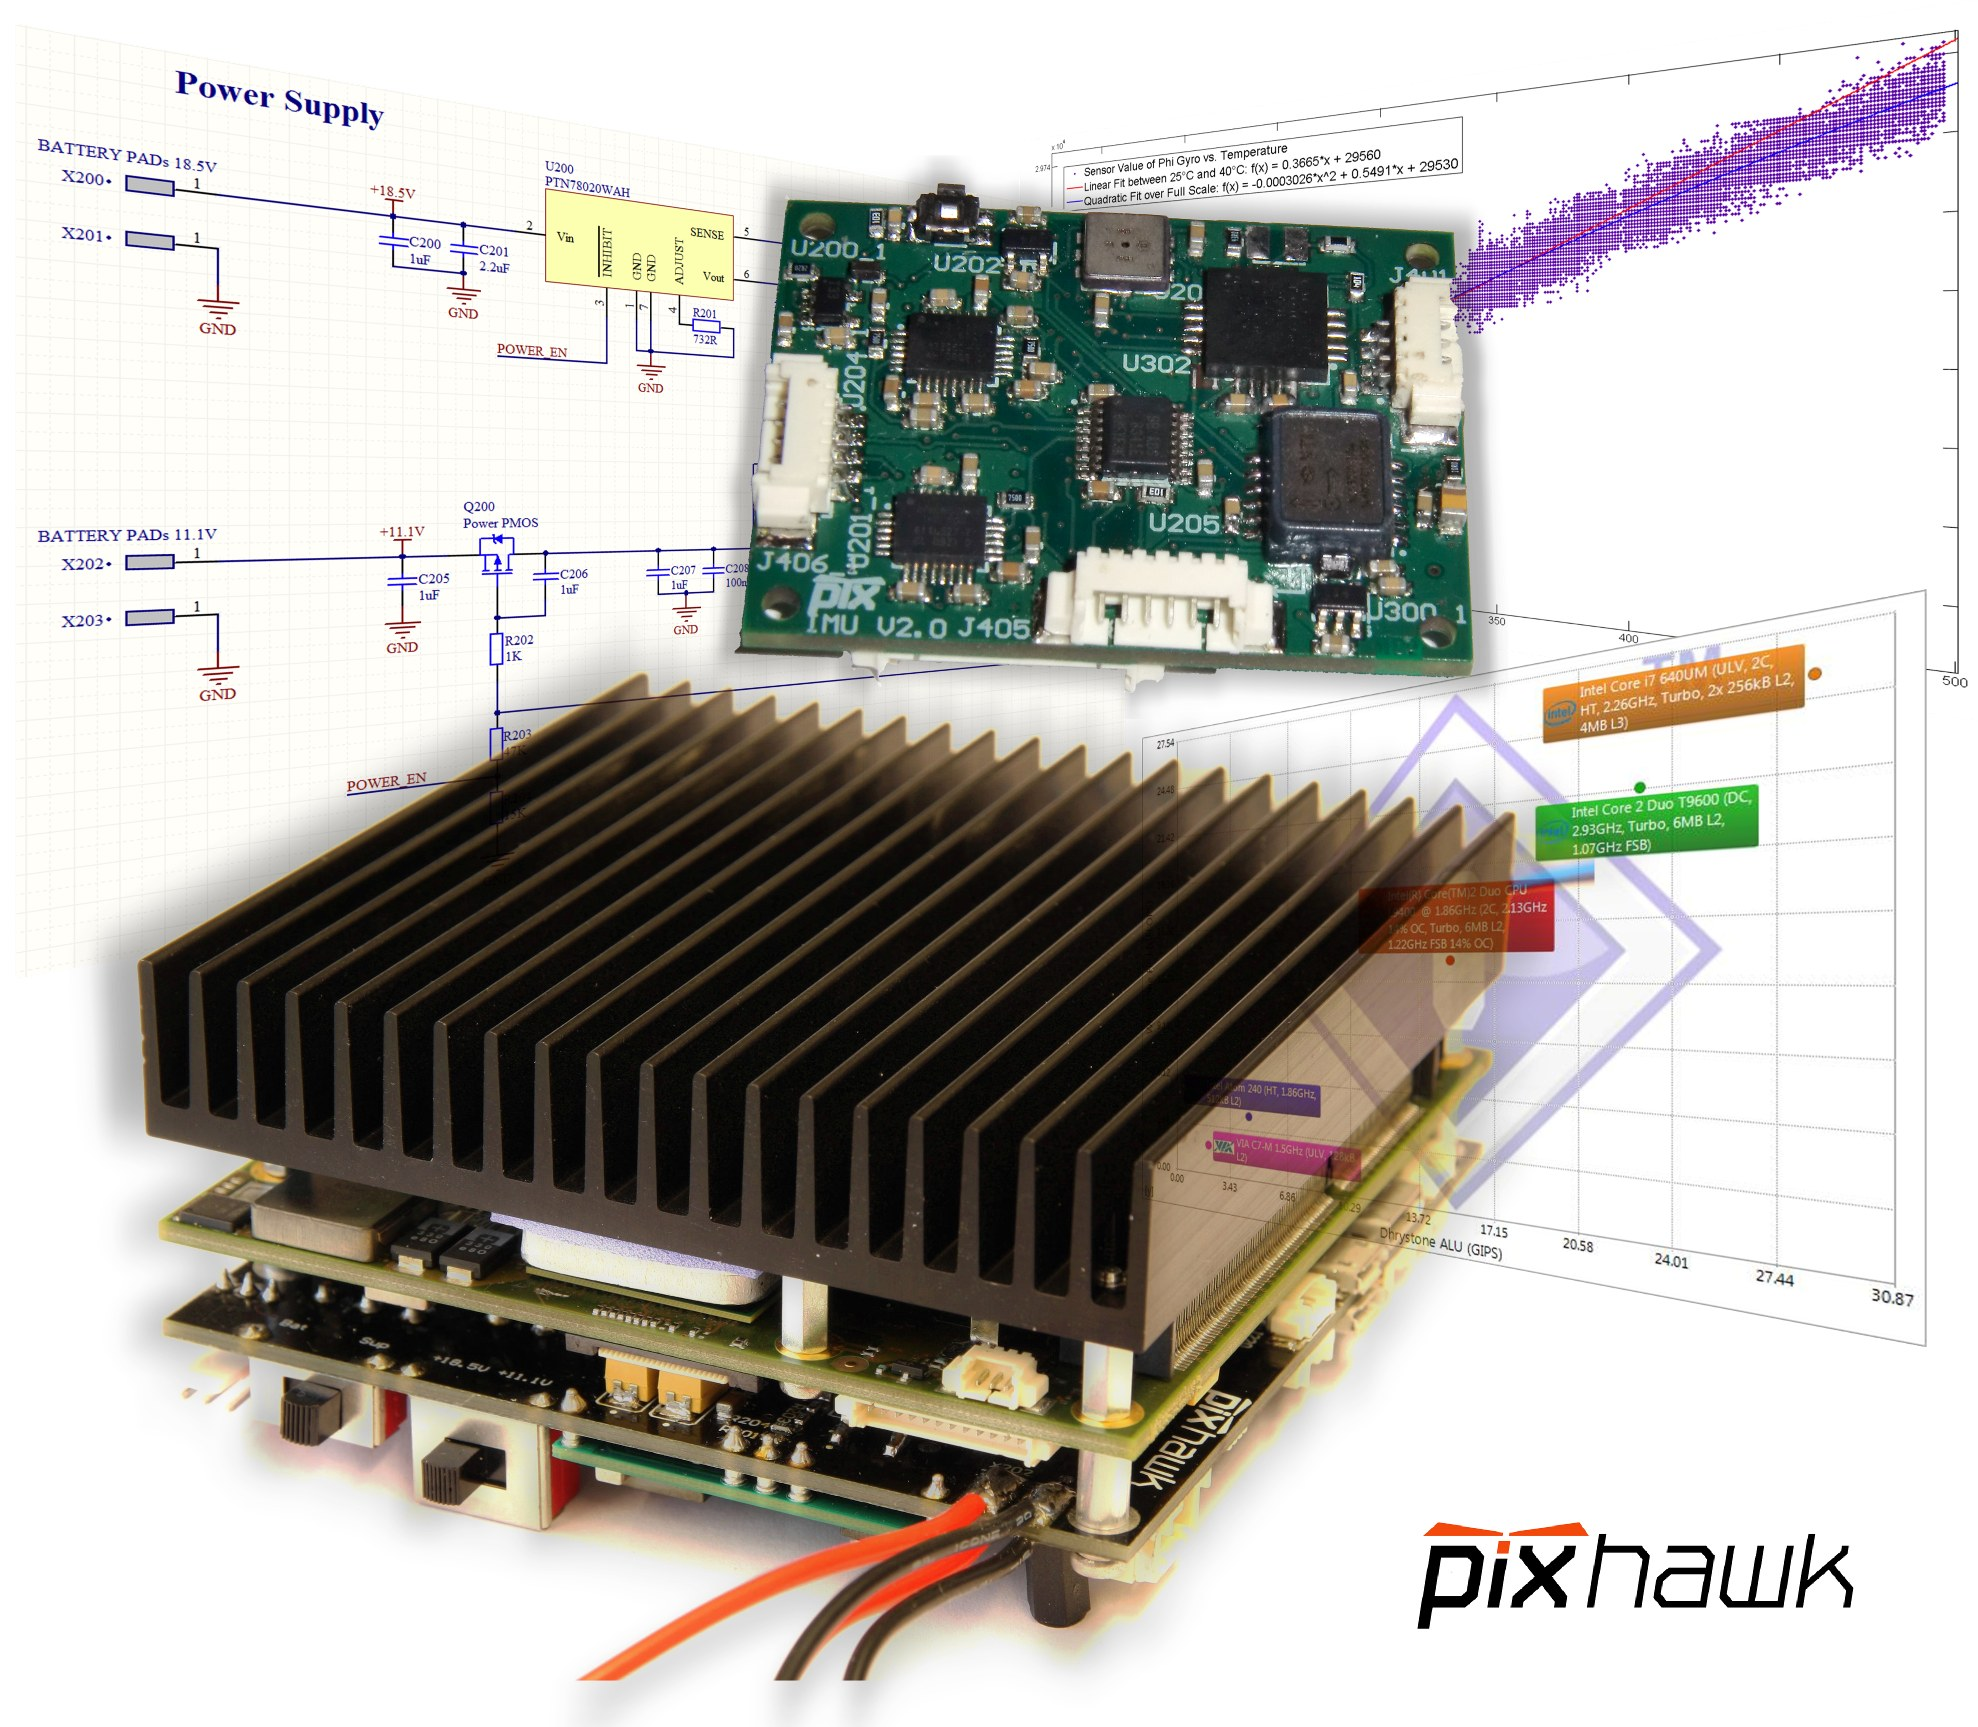
\includegraphics[width=0.9\textwidth]{titlepageimage.jpg}\\
\end{figure}

\begin{center}
  \vspace*{0.5cm}
  \Large
  \textit{Master Thesis CVG Lab\\SS 2017} \\
  \vspace{1cm}
  \Large \mdseries
  Daniel Keyes\\
  \vspace{0.5cm}
\end{center}

\begin{center}
    \rule{\linewidth}{0.5pt} \\
\end{center}

\Large

\begin{tabular}{l@{\hspace{0.5cm}}l}
  Advisors: 	& Federico Camposeco\\
  Professor: 	& Prof. Marc Pollefeys
\end{tabular}

\normalfont \normalsize

\clearemptydoublepage
\chapter{Abstract}

In any camera motion estimation pipeline, the problem of relocalization---determining where a camera is located in a previously constructed map---must be addressed to recover from tracking loss, minimize drift, and remain reliable over time. Whereas traditionally these maps have contained only a very sparse cloud of points, recent developments in visual odometry have shown that it is possible to generate a relatively dense point cloud while tracking camera motion. In this work, we leverage this rich geometric information to perform camera relocalization. We adopt approaches that were previously viable only with dedicated depth-sensing hardware; we analyze our results on two well-known relocalization benchmarks; and we analyze failure cases.

\clearemptydoublepage
\chapter{Acknowledgments}

Acknowledgments to people who supported you. In Semester theses this chapter can be removed.

\clearemptydoublepage

%list of contents, figures and tables
\phantomsection
\addcontentsline{toc}{chapter}{Contents}
\tableofcontents
\cleardoublepage
\phantomsection
\addcontentsline{toc}{chapter}{List of Figures}
\listoffigures
\cleardoublepage
\phantomsection
\addcontentsline{toc}{chapter}{List of Tables}
\listoftables
\cleardoublepage

%customize headers and footers
\pagestyle{fancyplain} % Chapter and Section appear in header
\renewcommand{\chaptermark}[1]{\markboth{#1}{}} % Changes chapter appearence
\renewcommand{\sectionmark}[1]{\markright{\thesection\ #1}} % Changes section appearence
\lhead[\fancyplain{}{\bfseries\thepage}]{\fancyplain{}{\bfseries\rightmark}}
\rhead[\fancyplain{}{\bfseries\leftmark}]{\fancyplain{}{\bfseries\thepage}}
%\cfoot{} % removes page number from footer
\cfoot[\fancyplain{}{}]{\fancyplain{\thepage}{}} %Page number in the first page of a chapter in footer 

%--------- include chapters----------------------------------------------
\mainmatter

\graphicspath{{introduction/}}

\chapter{Introduction}
\label{cha:introduction}

Finding correspondences between recent and formerly visited camera frames is a critical component in many computer vision and robotics systems. For the problem of simultaneous localization and mapping (SLAM), camera relocalization establishes loop closures, which are necessary to correct drift accumulated during the estimate. For applications which do not perform mapping, such as visual odometry (tracking camera movement from video), being able to relocalize is critical to recovering from tracking loss and returning to a known reference frame. This is also relevant to applications on low-power devices, such as mobile robotics or virtual and augmented reality on smartphones, in which it may be desirable to compute a high-quality map ahead of time and track against it later. In some use-cases, such as image retrieval, identifying the pose (i.e.\ the position and orientation) of the viewer in a known map is the goal itself.

In this thesis, we address the problem of relocalization using a recently developed measurement representation called ``semi-dense'' depth maps. In contrast to sparse depth maps, which only store a few nonzero values, and fully dense depth maps, which have a distance stored in every pixel, semi-dense depth maps record the depth of a \textit{significant fraction} of pixels. Recent developments in direct visual odometry \cite{engel2013semi} \cite{engel2017direct} \cite{Forster2014ICRA} have been able to achieve comparable results to depth-based methods, despite only using an RGB camera, and a recurring theme in these methods is the estimation of a semi-dense depth map in each frame. In these works, the maps contain a depth estimate at every pixel with a significant color gradient. This is in contrast to feature-based techniques \cite{klein2007parallel} \cite{murTRO2015}, which only track points located at peaks in the feature response space, and produce a comparatively sparse point cloud. In this thesis, we show how state-of-the-art RGB-D relocalization techniques can be re-applied RGB images paired with semi-dense depth maps.

Monocular (single camera) visual odometry itself comes with a variety of challenges. For example, depth estimation is indeterminate in the case of zero (or very little) camera translation. This can happen if a user rotates a camera around the camera center, perhaps to give a panoramic view of the scene. When camera translation resumes, if no original points are still visible within the viewing frustum, tracking is impossible. Additionally, in lieu of feature matching, direct techniques must make assumptions about camera motion to track pixels from frame to frame. They generally assume small camera movement, and only attempt to track points within a small radius, or (using a motion model) they might search on an epipolar line for the best point correspondence. These assumptions are violated in the case of fast or shaky camera movement, which is common in the real world and further motivates our problem.

Furthermore, these common sources of tracking failure are exacerbated by the scale ambiguity of video from a single camera. In the absence of inertial measurements or calibrated depth cameras, it is impossible to know the true size of observed objects. For example, in a typical structure-from-motion pipeline, the displacement between the initially chosen frames defines the scale. Because of this, multiple independent reconstructions of the same scene may be at arbitrarily different scales. In an on-line system, if tracking fails, we must recover both the original reference frame and the original scale of the scene.

In Chapter 2, we give an overview of related work. Chapter 3 gives a detailed description of the relocalization pipeline. This includes a summary of the visual odometry operation and depth map extraction techniques, as well as an overview of a typical image-based relocalization process. We further expound on techniques for descriptor learning and full \mbox{6-degree-of-freedom} camera localization. Chapter 4 presents concrete results on relocalization benchmarks, and we compare our work to prior visual and depth-based relocalization methods. We conclude in Chapter 5 with a discussion of future work, applications, limitations, and possible extensions to the method.

\cleardoublepage

\chapter{Method Overview}


% TODO: make a figure showing the pipeline as a flowchart

We perform relocalization in several steps. First, to create an initial map of a scene, we perform visual odometry using DSO on each of a set of training videos. For each training sequence, this yields a set of per-frame camera poses and estimated semi-dense point clouds, plus an adjacency list of frames with co-observed points. We then extract features from each keyframe; rather than using an explicit feature detector, we simply evaluate the descriptor at every defined pixel in the semi-dense depth map. In a second pass, we merge multiple keyframe observations of the same point by computing the mean descriptor value, as in [CITE TORSTEN'S PAPER].

In order to perform efficient retrieval of similar images, we compute an inverted index. We cluster features in the training set to create a visual word vocabulary and use the vocabulary to index training keyframes. We use the implementation of [CITE TORSTEN'S PAPER], which additionally filters results by their Hamming embeddings in order to remain descriminative while using a smaller visual vocabulary.

Finally, to relocalize, we compute descriptors for each frame in the test set, again at defined locations in the depth map. Note however that for the test set, we discard the depth information and do not compute the mean descriptor values, so that each test frame can be evaluated independently. Querying the inverted index now returns a list of plausible matches in the training set for each query frame in the test set. We then compute a set of feature correspondences between each training and test frame, which thereby can be used with a RANSAC Perspective-n-Point solver to find the query pose (in the training sequence's frame of reference). We perform geometric verification, i.e.\ compute poses from the top 50 retrieved images, and return the one with the most inlier correspondences.

\section{Visual Odometry}
-run DSO to get map (include algorithm? bookkeeping? note on how things are marginalized?)

\section{Feature Extraction}
In our experiments, we test two kinds of visual features. As a baseline, we use the well-known SIFT feature. We compare this to the learned features of [CITE TANNER'S PAPER], which has demonstrated state-of-the-art performance for use in camera relocalization.

In practice, to extract SIFT features, we first detect a large quantity of SIFT keypoints. Then, for each depth pixel, the closest SIFT keypoint within a small radius ($r=3$ pixels) is assigned. This can be efficiently implemented by, for example, binning features detected in the image into $r \times r$ squares and only checking adjacent bins. After performing this process, some depth pixels may be discarded, e.g.\ if they are not near a peak in the SIFT feature response space, and vice versa.

In contrast to this, it seems reasonable to train a dense descriptor (DEFINE WHAT THAT MEANS), so that we can evaluate it at any point in a semi-dense depth map by simply sampling a pixel of the dense descriptor. TODO: GIVE OVERVIEW OF TANNER'S PAPER

\section{Training a Visual Vocabulary}
	
-for all training images, do clustering
	-approximate clustering
	-assign to clusters

\section{Building the Inverted Index}
-create visual words database
	-description of torsten's stuff? hamming embeddings? inverted index? visual words voting? normalization?


-image matching
	-ratio test. maybe some pseudocode? reference to lowe's paper?
-geometric verification
	-space for PnP derivation? or the definition at least?
-alignment onto original VO and onto GT trajectories
	-sim3 alignment
	-computing relative camera pose, rescaling transformation

\chapter{Experiments}




\backmatter

%Bibliography
%\bibliographystyle{IEEEtran}		% use this for electric engineering thesis (contains support for datasheets)
\bibliographystyle{splncs}		% use this for computer vision thesis
\bibliography{thesis}
\cleardoublepage

%\appendix
%\include{appendix/appendix}

\end{document}
